\documentclass[a4paper,12pt]{article}


% % % % % % % % % % % % % % % % % % % % % % % % % % % % %
% % ATTENTION : dans les figures le label doit être mis 
%APRES le caption pour que le numéro de la figure lorqu'on
%la référence soit le bon ; sinon on a le numéro du paragraphe
% % % % % % % % % % % % % % % % % % % % % % % % % % % % %

% package qui fournit \justify 
\usepackage[document]{ragged2e}

%pifont pour les puces de formes spéciales
\usepackage{pifont}
\usepackage[table]{xcolor}
\usepackage{tabu}
% césure exemple
% \hyphenation{an-ti-cons-ti-tu-tion-nel

\usepackage[utf8x]{inputenc}
\usepackage[T1]{fontenc}
\usepackage[frenchb]{babel} % If you write in French
%\usepackage[english]{babel} % If you write in English
\usepackage{lmodern} % Pour changer le pack de police
\renewcommand*\familydefault{\sfdefault}
\usepackage{makeidx}
\usepackage{amsthm}
\usepackage{amsmath}
\usepackage{amssymb}
\usepackage{mathrsfs}
\usepackage{stmaryrd}
\usepackage{geometry}
%\usepackage{graphicx}
\usepackage{graphbox}
\usepackage{supertabular}
\usepackage{tabularx}
\usepackage{longtable}
\usepackage{pdflscape}
\geometry{hmargin=2cm,vmargin=2cm}

\usepackage{booktabs}
\usepackage{tabularx}
\usepackage[table]{xcolor}
\usepackage{ltablex}
\usepackage{float}
\usepackage{url}

\usepackage{chngcntr}
\counterwithin*{footnote}{page}


\usepackage[titletoc,toc,title,page]{appendix}
\renewcommand{\appendixtocname}{Annexes}
\renewcommand{\appendixpagename}{Annexes}

\usepackage{standalone}
\usepackage{ifthen}
\usepackage{xstring}
\usepackage{calc}
\usepackage{pgfopts}
\usepackage{tikz}
\usetikzlibrary{positioning,shapes,shadows,arrows}
%\usepackage{array,ragged2e}
\usepackage{algpseudocode}
\usepackage{algorithm}
\makeatletter
\renewcommand{\ALG@name}{Algorithme}
\renewcommand{\listalgorithmname}{Table des algorithmes}

\newtheorem{theo}{Définition}[section]
\usepackage{mathtools, bm}
\usepackage{amssymb, bm}

\usepackage{hyperref}
\hypersetup{
    colorlinks=true,       % false: boxed links; true: colored links
    linkcolor=black,       % color of internal links
    citecolor=purple,       % color of links to bibliography
    urlcolor=blue          % color of external links
}

\usepackage{listings}

\definecolor{dkgreen}{rgb}{0,.6,0}
\definecolor{dkblue}{rgb}{0,0,.6}
\definecolor{dkyellow}{cmyk}{0,0,.8,.3}

\lstset{
  language        = php,
  basicstyle      = \small\ttfamily,
  keywordstyle    = \color{dkblue},
  stringstyle     = \color{red},
  identifierstyle = \color{dkgreen},
  commentstyle    = \color{gray},
  emph            =[1]{php},
  emphstyle       =[1]\color{black},
  emph            =[2]{if,and,or,else},
  emphstyle       =[2]\color{dkyellow}}



\usepackage{blindtext}
\usepackage{enumitem} % pour changer les puces dans \itemize


\date{\today}

\makeindex
\def\siecle#1{\textsc{\romannumeral #1}\textsuperscript{e}}
\newcommand{\argmax}{\mathop{\mathrm{argmax}}\nolimits}
\newcommand{\pgcd}{\mathop{\mathrm{pgcd}}\nolimits}

\makeatletter
\renewcommand{\pod}[1]{\allowbreak\mathchoice
  {\if@display \mkern 18mu\else \mkern 8mu\fi (#1)}
  {\if@display \mkern 18mu\else \mkern 8mu\fi (#1)}
  {\mkern4mu(#1)}
  {\mkern4mu(#1)}
}

\usepackage{wallpaper}
%\usepackage{bsymb,b2latex}

\begin{document}
\renewcommand{\labelitemi}{\textbullet}
% pour factoriser l'échelle des figures 
%utilisation scale=\scaledvwa au lieu de scale = 0.3 ... 
\newcommand{\scaledvwa}{0.4} 
\newcommand{\scaledvw}{0.3}
\newcommand{\scalekad}{0.45}


\phantomsection
\begin{titlepage}
	\parindent=0pt
\ThisTileWallPaper{1.3\paperwidth}{1.0\paperheight}{images/couv1}
 
\addtolength{\wpXoffset}{-4.5cm}

%	\vspace*{\stretch{1}}
%	\begin{center}
%		
\includegraphics[scale=0.5]{images/enac.png}%
%	\end{center}
	
\color{white}{	\vspace*{\stretch{1}} }
	\hrulefill
	\begin{center}\bfseries\Huge
		\color{white}
		{Optimisation Combinatoire Avancée : Etude de l'article "Benders Decomposition for Large-Scale Uncapacitated Hub Location"} 
	\end{center}
	\hrulefill
	
	\vspace*{1cm}
	\begin{center}\bfseries\Large
			\color{white}
		{Felix QUINTON - Abdelkader BELDJILALI}
		
	\end{center}
	
	\vspace*{\stretch{2}}


\end{titlepage}
%on créé la couverture

\pagebreak

\tableofcontents
\pagebreak
\justify

\pagebreak

\section*{Introduction}
\addcontentsline{toc}{section}{Introduction}

%Parmi les problèmes d'optimisation combinatoire, on peut distinguer 4 grandes classes principales.
%
%\begin{enumerate}
%	\item Les problèmes de chargement de type knapsack (KP)
%	\item Les problèmes de tournée de véhicules \textit{Vehicule Routing Problems} (VRP) dont un cas particulier est le problème voyageur de commerce (TSP)
%	\item Les problèmes de couverture :  \textit{Set Covering Problems} (SCP)
%	\item Les problèmes de localisation : \textit{Facility Location Problems} (FLP)
%	\end{enumerate}

L'article étudié, \cite [\textit{Benders Decomposition for Large-Scale Uncapacitated Hub Location}]{ccl}, présente un algorithme exact qui permet de traiter des instances impliquant jusqu'à 500 noeuds et 250 000 types de marchandises transportées. Pour ce faire, une décomposition de Benders améliorée par divers techniques est utilisée pour en augmenter l'efficacité et la robustesse. 

 
 





\section{Problématique générale}

La problématique générale de l'article étudié est de développer un algorithme exact pour la résolution de grande instance du problème de localisation UHLPMA.

%\subsection{}
%\paragraph{}

%\subsection{Description du système et de son environnement}
%\begin{figure}[H]
%	\begin{center}	
%		\includegraphics[scale=0.3]{images/0/ctx}
%		\caption{Environnement du système}
%		\label{ctx}
%	\end{center}
%\end{figure}



\section{Modèle complet}

En partant du modèle de Hamacher et al. \cite[Adapting polyhedral properties from facility to hub location problems (2004)]{hln}, les auteurs ont défini un ensemble $E_k$ d'arêtes $e$ d'extrémités identiques ou différentes. Ces extrémités sont candidates à devenir des hub pour chaque bien k. L'amélioration réside dans le fait que $E_k$ réduit le choix des hubs potentiels contenus dans H d'où le problème (P) ci-dessous qui exploite les propriétés spécifiques des solutions optimales du problème UHLPMA. C'est ce problème original (P) que les auteurs résolvent en partitionnant les variables (décomposition de Benders) : 

\[ \min \sum_{i \in H}f_iz_i + \sum_{k \in K}\sum_{e \in E_k}F_{ek}x_{ek}\]
tel que
\begin{subequations}
    \begin{align}
        \sum_{e \in E_k}x_{ek} = 1, \quad &\forall{k\in K}&\\
        \sum_{e \in E_k:i\in e}x_{ek} \le z_i,\quad &\forall{i \in H}, \forall{k\in K}&\\
        x_{ek} \ge 0, \quad &\forall{k \in K}, \forall{e \in E_k}&\\
        z_i\in \{0,1\},\quad &\forall{ i \in H}&
    \end{align}
\end{subequations}
 où $H$ est l'ensemble des localisations possibles pour un hub, $K$ est l'ensemble des biens qui doivent être acheminés, $f_i$ est le coût fixe de transformation en hub d'un n\oe ud $i\in H$, $z_i$ est une variable binaire égale à 1 si le n\oe ud $i$ est un hub, et à 0 sinon, $F_{ek}$ est le coût de transport non orienté pour un arc du graphe $e \in H\times H$ et un bien $k \in K$, et $x_{ek}$ est un variable binaire égale à 1 si le bien $k \in K$ transite par l'arc $e \in H\times H$ et à 0 sinon.
 
 Le coût de transport non orienté pour un arc $e = (i,j) \in H\times H$ est le minimum du coût de transport dans le sens $i \rightarrow j$ et du coût de transport dans le sens $j \rightarrow i$, c'est à dire $F_{ek} = \min \{ \hat{F}_{ijk};\hat{F}_{jik}\}$.



\section{Décomposition réalisée}

Problème primal :

\[ \min \sum_{e \in E_k}\sum_{k \in K}F_{ek}x_{ek}\]
tel que
\begin{subequations}
    \begin{align}
        \sum_{e \in E_k}x_{ek} = 1, \quad &\forall{k\in K}&\\
        x_{ek} \ge 0, \quad &\forall{k \in K}, \forall{e \in E_k} \label{eq1}&\\
        \sum_{e \in E_k:i\in e}x_{ek} \le \hat{z}_i,\quad &\forall{i \in H}, \forall{k\in K}\label{eq2}&\\
    \end{align}
\end{subequations}

où $\hat{z}$ est un vecteur fixé dans l'ensemble des vecteurs binaires associés aux variables $z_i$.

\smallskip

Problème dual :

\[ \max \sum_{k \in K}\alpha_k - \sum_{i \in H}\sum_{k \in K} \hat{z}_iu_{ik}\]
tel que
\begin{subequations}
    \begin{align}
        \alpha_k - u_{e_1k} - u_{e_2k} \le F_{ek}, \quad &\forall{k\in K}, \forall{e \in E}, |e| = 2&\\
        \alpha_k - u_{e_1k} \le F_{ek}, \quad &\forall{k\in K}, \forall{e \in E}, |e| = 1&\\
        u_ik \ge 0, \quad &\forall{i \in H}, \forall{k \in K}
    \end{align}
\end{subequations}

où $\alpha_k, k\in K$ sont les variables associées aux contraintes \ref{eq1} et $u_{ik}, i \in H, k \in K$ les variables associées aux contraintes \ref{eq2}

\smallskip

Problème maître :

\[ \min \sum_{i \in H} f_iz_i + \eta\]
tel que
\begin{subequations}
    \begin{align}
       \eta \ge \sum_{k \in K}\alpha_k - \sum_{i \in H}\sum_{k \in K} z_iu_{ik}, \quad &\forall{(\alpha,u) \in P_D}&\\
       \sum_{i \in H} z_i \ge 1 \quad &&\\
        z_i \in \{0,1\}, \quad & \forall{i \in H}&
    \end{align}
\end{subequations}
	

	

\section{Résolution des problèmes}

\paragraph{Résolution du problème (P) :}La reformulation de Benders précédente contient un nombre exponentielle de contraintes. Les auteurs ont donc résolu itérativement le problème maître réduit (PMR) contenant un faible nombre de contraintes (4a) associées aux points extrêmes dans $P_D$. Les contraintes sont ajoutées au fur et à mesure en résolvant les sous-problèmes duaux jusqu'à atteindre une solution optimale du problème original (P) comme indiqué dans le pseudo-code  figure \ref{alg1}.

\begin{itemize}
	\item ub désigne une borne supérieure,
	\item t : Entier caractérise les itérations successives,
	\item $P^t_D$ : Ensemble des points extrême à l'itération t, 
	\item  $MP(P^t_D)$ : Problème Maître relaxé (PMR) en remplaçant $P_D$ par $P^t_D$,
	\item $v(MP(P^t_D)$ : Valeur optimale du (PMR) à l'itération t,
	\item $z^t$ : Vecteur optimal à l'itération t,
	\item $DS(z^t)$ : Sous-problème dual (SD) pour $z^t$,
	\item $v(DS(z^t))$ : Valeur optimale du sous-problème (SD).
\end{itemize}

\begin{figure}[H]
	\begin{center}	
		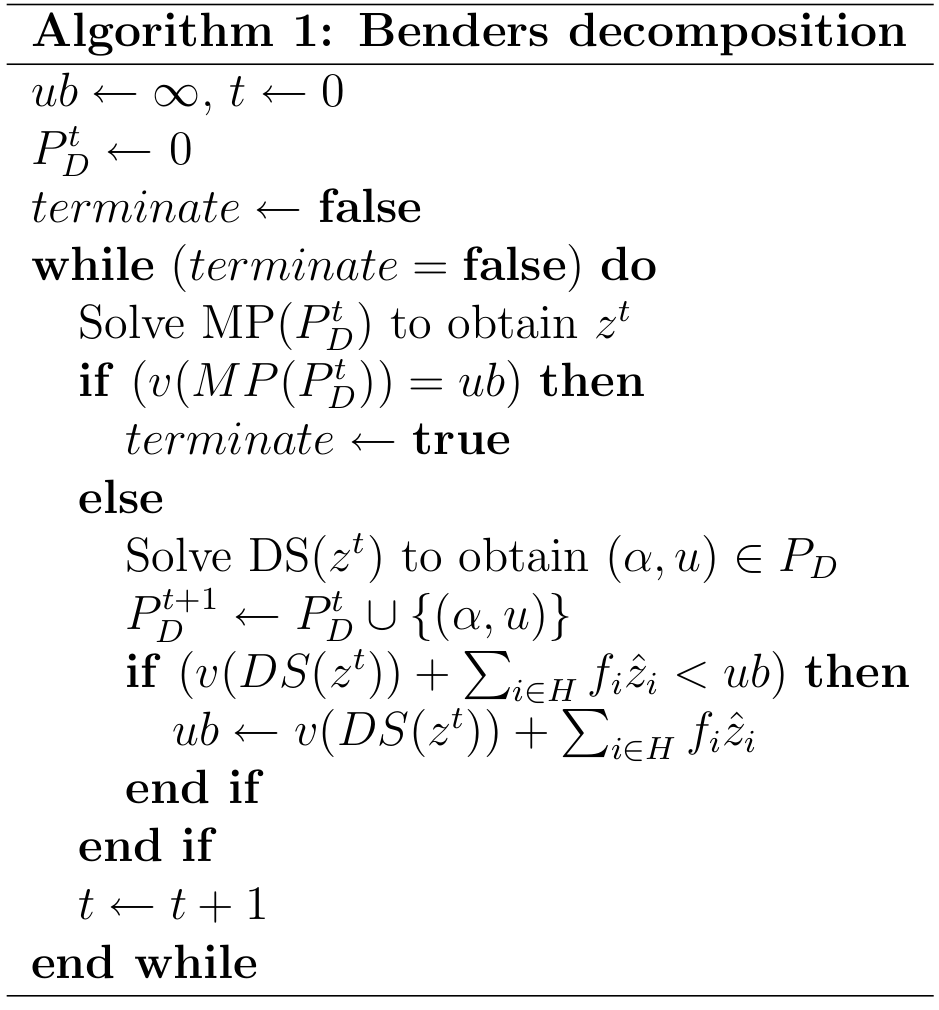
\includegraphics[scale=0.3]{images/alg1}
		\caption{Calcul de la solution optimale du problème original (P) si elle existe.}
		\label{alg1}
	\end{center}
\end{figure}


  \paragraph{Résolution de sous-problème Dual :}

L'algorithme précédent nécessite la résolution des sous-problèmes duaux $DS(z^t)$. Les auteurs utilisent une méthode qui exploite la structure du sous-problème primal en l'occurence sa \textit{décomposabilité} en card(K) sous-problèmes $PS^t_k $ plutôt qu'une résolution directe du dual à l'aide d'un solveur. Les solutions du dual $(\alpha^t, u^t)$ sont déduites du théorème complémentaire en théorie de la dualité. Ainsi à partir d'une solution optimale $x^t$ du primal $PS^t_k$, les auteurs en déduisent un ensemble noté $DO^t$ de solutions optimales du dual $DS^t$.

\paragraph{}Il s'agissait ensuite pour les auteurs de sélectionner une solution optimale $(\alpha^t, u^t)$ tirée de $DO^t$, notamment en sélectionnnant des valeurs admissibles pour les variables duales $\alpha^t_k$ et $u^t_{ek}$. Des conditions filtrantes sont aussi déterminées, en particulier, une borne inférieure des variables $u_{ik}$ notée $l_{ik}$.
Enfin, les auteurs privilégient le choix d'un vecteur dual optimal $(\alpha^t, u^t)$ qui
produira des coupes efficaces d'optimalité, en l'occurrence les vecteurs dont $u^t$ est le plus petit possible pour obtenir la plus grande borne inférieure possible pour la valeur optimale du problème maître relaxé à l'itération suivante $t+1$.


\section{Techniques d’amélioration de l'algorithme}


\paragraph{Reformulation multicoupe : }
Cette technique décompose le problème maître en $|H|$ sous-problèmes indépendants, un pour chaque n\oe ud. Seules $|H|$ coupes d'optimalité sont générées à partir de chaque polyèdre dual associé au sous-problème $j$ contre $|K|$ si la décomposition complète des sous-problèmes duaux avait été utilisée. Auquel cas, les $|K|$ coupes par itération auraient été contre productives en terme de temps de calcul.


\[ \min \sum_{i \in H} f_iz_i + \sum_{i \in H} \eta_i  \]
tel que
\begin{subequations}
	\begin{align}
	\eta_j \ge \sum_{k \in K_j}\alpha_k - \sum_{i \in H}\sum_{k \in K_j} z_iu_{ik} \quad &\forall j \in H, \forall{(\alpha,u) \in P_{D^j}}&\\
	\sum_{i \in H} z_i \ge 1 \quad &&\\
	z_i \in \{0,1\}, \quad & \forall{i \in H}&
	\end{align}
\end{subequations}

\paragraph{Coupe Pareto-optimale : }
Les auteurs ont utilisé ici la méthode de Magnanti et Wong \cite[1981]{mw} pour obtenir des coupes non dominées plus efficaces et ainsi améliorer la convergence.

\paragraph{Tests d'élimination : }
Ici, l'efficacité et la convergence de l'algorithme de décomposition de Benders sont améliorées en réduisant la taille du modèle original. Les auteurs ont utilisés deux tests
visant à éliminer des n\oe ud de l'ensemble $H$ et dont on sait, compte tenu des informations acquises lors des itérations, qu'elles ne pourront pas apparaître dans la solution optimale à la manière d'un Branch\&Bound.


\paragraph{Heuristique : }
\section{les grandes lignes des résultats obtenus (taille des problèmes, temps de calcul)} 

\section{Conclusion}
%\addcontentsline{toc}{section}{Conclusion}

Les auteurs ont utilisé avec succès une décomposition de benders améliorée pour résoudre des instances du problème UHLPMA contenant jusqu'à 500 noeuds et 250 000 marchandises à acheminer via un sous-réseau de hubs. Ce qui constitue probablement un record à la date de rédaction de l'article en juin 2010.


%\pagebreak
%\listoffigures
%\pagebreak
%\listoftables
%\newpage
%\appendix
%\section{Annexe}
\label{annexe_A}

\begin{itemize}
\item Pour écrire simplement les clés sur le disque, nous utilisons Marshal, qui garantit la compatibilité entre toutes les plateformes pour une même version de OCaml.
\item Bien que BatIO propose une API pour manipuler les canaux au niveau du bit, nous avons préféré rester au niveau de l'octet car il s'agit d'une solution plus évolutive – rares sont les bibliothèques proposant ce genre de fonctions. D'ailleurs, son fonctionnement est identique à ce que nous implémentons, reposant sur une lecture octet par octet.
\item Dans la version actuelle du code, les canaux d'entrées-sorties ne sont pas toujours fermés proprement lorsqu'une exception « fatale » est rencontrée…
\item Les blocs chiffrés sont écrits sur le canal de sortie sous forme de chaîne de caractères. Ainsi, le message chiffré constitué de deux blocs « 1234 5678 » est écrit, sous forme hexadécimale, «~31 32 33 34 00 35 36 37 38 00~». Pour déchiffrer, on lit donc le canal d'entrée « chaîne par chaîne ». Cela a l'avantage de produire une sortie lisible mais présente l'inconvénient de consommer bien plus d'espace qu'une représentation binaire qui serait spécialement conçue pour le problème.
\end{itemize}

%\section{Annexe}
\label{annexe_A}

\begin{itemize}
\item Pour écrire simplement les clés sur le disque, nous utilisons Marshal, qui garantit la compatibilité entre toutes les plateformes pour une même version de OCaml.
\item Bien que BatIO propose une API pour manipuler les canaux au niveau du bit, nous avons préféré rester au niveau de l'octet car il s'agit d'une solution plus évolutive – rares sont les bibliothèques proposant ce genre de fonctions. D'ailleurs, son fonctionnement est identique à ce que nous implémentons, reposant sur une lecture octet par octet.
\item Dans la version actuelle du code, les canaux d'entrées-sorties ne sont pas toujours fermés proprement lorsqu'une exception « fatale » est rencontrée…
\item Les blocs chiffrés sont écrits sur le canal de sortie sous forme de chaîne de caractères. Ainsi, le message chiffré constitué de deux blocs « 1234 5678 » est écrit, sous forme hexadécimale, «~31 32 33 34 00 35 36 37 38 00~». Pour déchiffrer, on lit donc le canal d'entrée « chaîne par chaîne ». Cela a l'avantage de produire une sortie lisible mais présente l'inconvénient de consommer bien plus d'espace qu'une représentation binaire qui serait spécialement conçue pour le problème.
\end{itemize}


\newpage
\nocite{*}  %affiche toutes les entrées du bib même celles qui ne sont pas citées.
% cf.    http://www.tuteurs.ens.fr/logiciels/latex/bibtex.html
% compilation en TROIS PHASE  bibtex traite un fichier *.aux mais bibtex mon_fichier comme bibtex mon_fichier.aux sont acceptés 
% latex mon_fichier.tex
% bibtex mon_fichier
% latex mon_fichier.tex


%\renewcommand{\bibname}{references.bib}
% ou
\renewcommand{\refname}{Bibliographie}
% dans le préambule.
\bibliography{references}
\bibliographystyle{alpha}

%\pagebreak

\subsubsection*{}
\pagebreak
\thispagestyle{empty}
\ThisTileWallPaper{1.45\paperwidth}{1.0\paperheight}{images/couv1}
\addtolength{\wpXoffset}{-4.5cm}


\justify








\end{document}
